% Behaviour of the stator voltage and the RMS-value of the stator
% flux as a function of speed in scalar control.
% Author: Erno Pentzin (2013)
\documentclass{article}
\usepackage{amsmath} % Required for \varPsi below
\usepackage{tikz}
\begin{document}

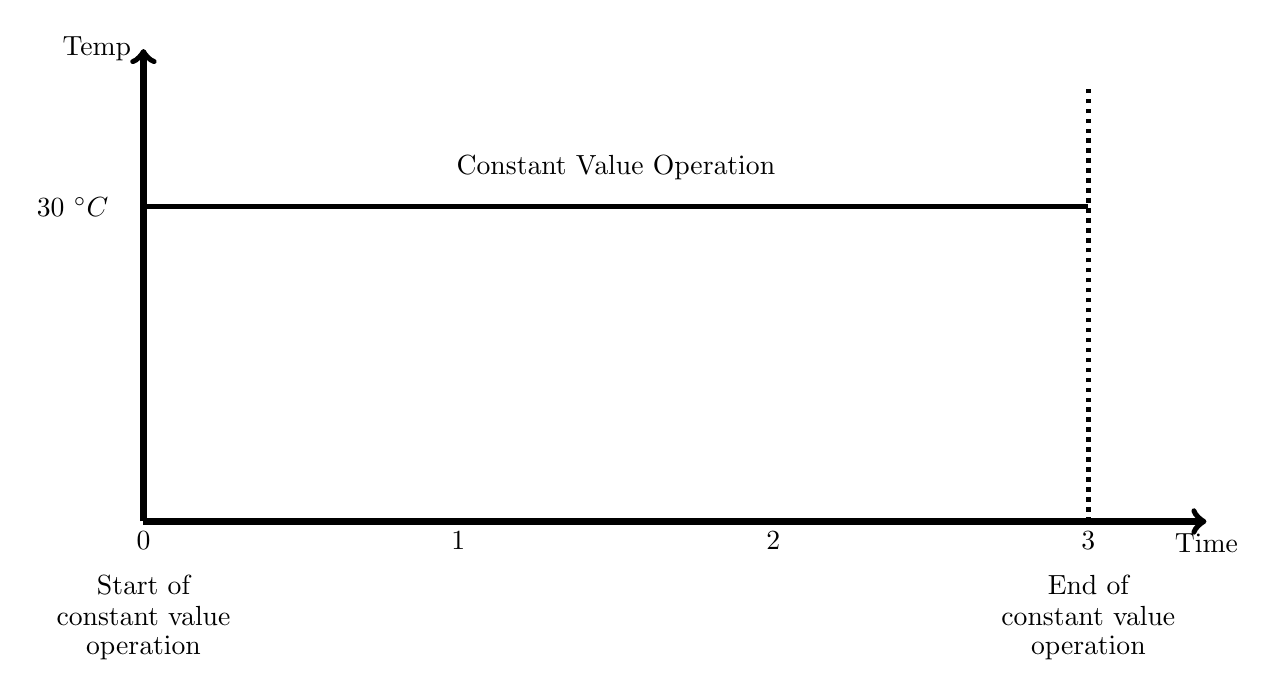
\begin{tikzpicture} [scale=2]

% horizontal axis
\draw [->, line width=0.8mm] (0,0) -- (6.75,0) node[anchor=north] {Time};
% labels
\draw	(0,0) node[anchor=north] {0}
		(2,0) node[anchor=north] {1}
		(4,0) node[anchor=north] {2}
		(6,0) node[anchor=north] {3};
% ranges
\draw	%(1,3.5) node{{\scriptsize Constant flux}}
		(3,2.25) node{{Constant Value Operation}};

% vertical axis
\draw [->, line width=0.8mm] (0,0) -- (0,3) node[anchor=east] {Temp};
% nominal speed
\draw [dotted, ultra thick] (6,0) -- (6,2.75);

% Us
\draw [ultra thick] (0,2) -- (2,2) -- (6,2);
\draw [line width=3]  (-0.45,2) node {30 $ ^{\circ} C$}; %label
\draw [line width=1] (0,-0.4) node {Start of}; %label
\draw [line width=1] (0,-0.6) node {constant value}; %label
\draw [line width=1] (0,-0.8) node {operation}; %label
\draw [line width=2] (6,-0.4) node {End of}; %label
\draw [line width=2] (6,-0.6) node {constant value}; %label
\draw [line width=2] (6,-0.8) node {operation}; %label
%\draw (1,1.5) node {$U_s$}; %label

% Psis
%\draw[thick,dashed] (0,3) -- (2,3) parabola[bend at end] (6,1);
%\draw (2.5,3) node {$\varPsi_s$}; %label

\end{tikzpicture}

\end{document}
